% !TeX root = ../../main.tex
% Add the above to each chapter to make compiling the PDF easier in some editors.

\section{IOG}\label{ord:ch3:sec1}

The paper "Interactive Object Segmentation with Inside-Outside-Guidance" published by Zhang et. al in 2020 provides a state-of-the-art method to perform interactive object segmentation \cite{Zha2020}.

\subsection{Method Description}\label{ord:ch3:sec1:subsec1}
The execution of this method delivers a binary segmentation result of one object in an image. 
To segment multiple objects in one image, the methods requires multiple executions.

As interactive methods IOG requires a user input in the form of three mouse-clicks on fore- and background of the input image, the procedure is the following: 
First, in order to form an "almost-tight bounding box"\cite{Zha2020} two exterior clicks are set at the corner locations of the object (top-left and bottom-right or bottom-left and top-right).
Based on these two points the other two corner points are derived, which leads to four points on the background. 
Second, to define the object inside the bounding box a single click around the center of the desired object is made, this click will be processed as foreground point. 
The background points "provide "outside" guidance (indicating the background regions) while the interior click gives an "inside" guidance (indicating the foreground region), thus giving the name \textit{Inside-Outside-Guidance}"\cite{Zha2020}.

These three points are preprocessed before applying to the actual model. To include context from the surrounding region the bounding box is enlarged by several pixels. 
In order to focus on the target of interest the enlarged bounding box is cropped and resized to the size of 512x512 pixels. 
For background and foreground points, a separate heatmap is created by centering a 2D Gaussian around each point. 
The two heatmaps have the size of 512x512 pixels as well and are concatenated with the input RGB image to create a 5 channel input for the model. 

\begin{figure}
	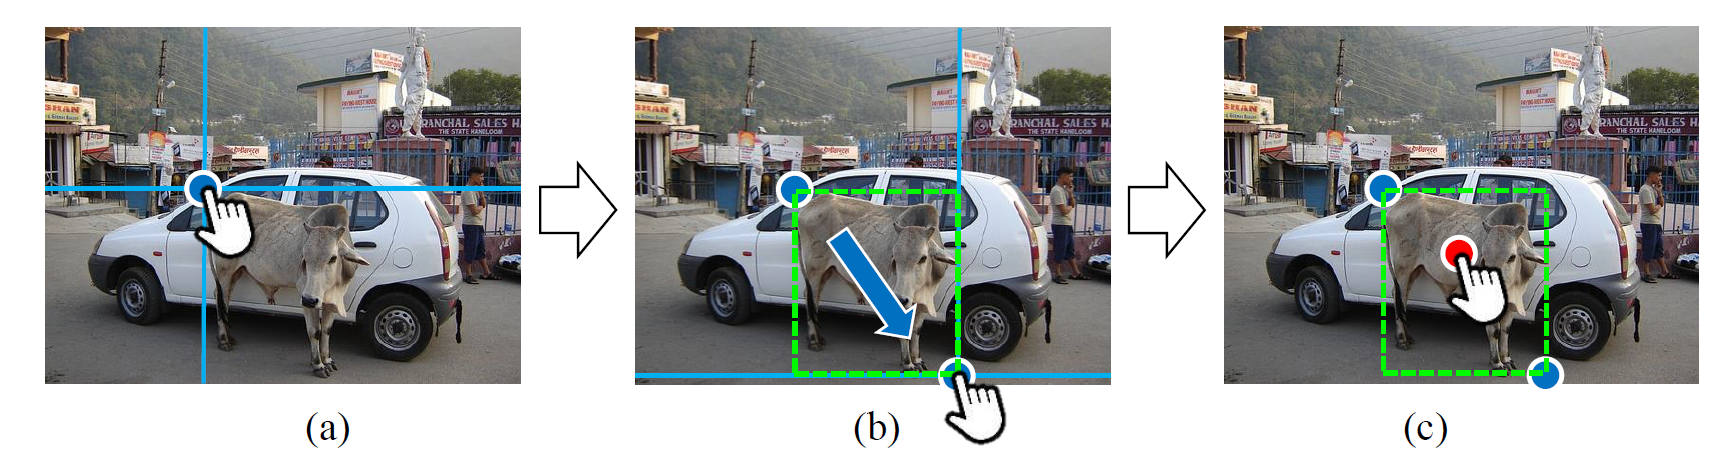
\includegraphics[width=\linewidth]{figures/chap31_clicks.png}
	\caption{Inside-Outside guidance.}
	\label{fig:ch3:sec1:iog}
\end{figure}

\subsection{Architecture}\label{ord:ch3:sec1:subsec2}

The architecture of the IOG method is based on a "coarse-to-fine design" \cite{Zha2020} (see Figure \ref{fig:ch3:sec1:arch}), containing two main parts: the CoarseNet and the FineNet.

\paragraph{CoarseNet}
The CoarseNet contains the heavy encoder part, also refereed as backbone, for what a ResNet-101 is used. 
This ResNet-101 is implemented with out a head of fully connected layers, but ends with the casual ResNet blocks. 
After the backbone a PSP-network is applied in order to enrich "the representation with global contextual information"\cite{Zha2020}.
The coarse prediction from the PSP-Net has a of shape of 32x32 pixels with 512 feature maps. 
From this on the layers are enlarged by a four staged upsampling process to obtain the original input size of 512x512 pixels. 
During the upsampling process activations from the residual parts of the ResNet are transferred from the ResNet using so lateral connections and concatenated with the upsampled layers. 
This is advantageous due to the combinations of localization detail from the several ResNet layers with the deeply processed activations from the PSP-net.

\paragraph{FineNet}
The FineNet is based on a multi-scale fusion structure. 
The activations from all four stages of the upsampling process from the CoarseNet are further processed in different paths. 
In most of them additional convolution and upsampling operations are applied in order to pressure "features at deeper layers for better trade-off between accuracy and efficiency" \cite{Zha2020}.
These different paths are concatenated to create the final prediction in the form of a probability map.
The FineNet allows to recover a more precise segmentation prediction, due to the combination of activations from multiple layers. 
\\
This architecture especially stands out due to its application of lateral connection from different levels in order to recover local detail. 
Especially, the combination of layers with high localization detail with the layers, that contain high detection details, is precious in order to prevent the loss of information during the process of down- and upsampling.

\begin{figure}
	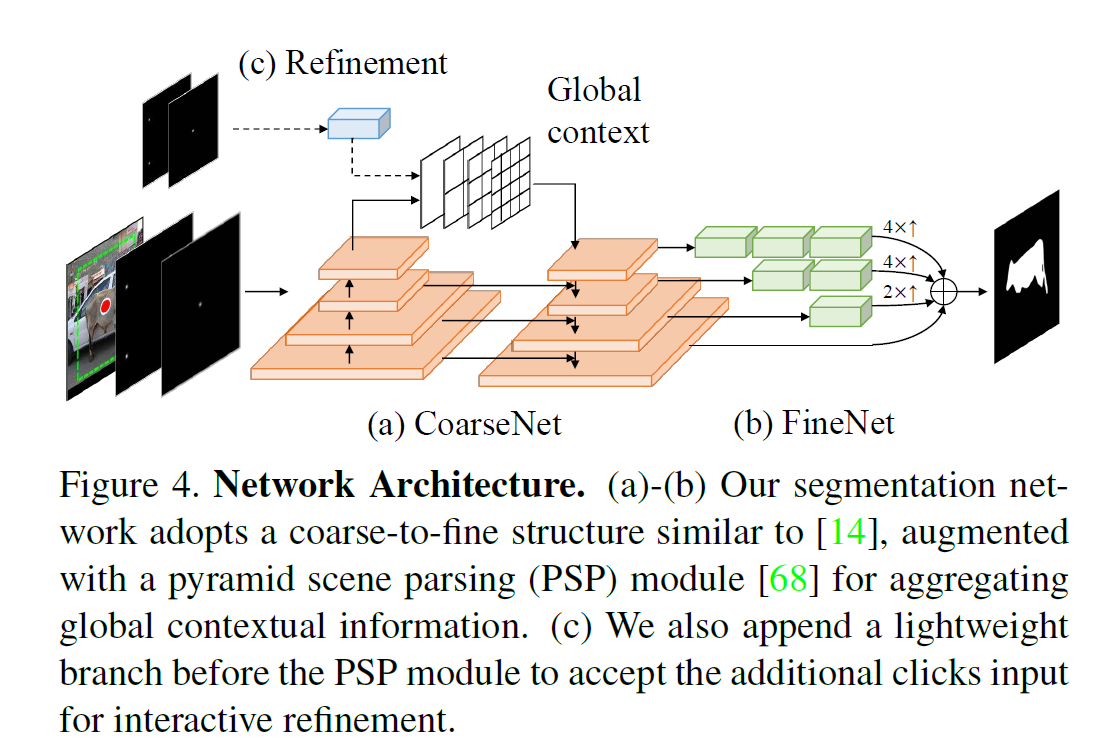
\includegraphics[width=\linewidth]{figures/chap31_arch.png}
	\caption{IOG architecture.}
	\label{fig:ch3:sec1:arch}
\end{figure}

\subsection{Refinement}\label{ord:ch3:sec1:subsec3}
For the case a segmentation results does not meet the users expectations a refinement can be performed several times. 
This is realized by obtaining an additional click from the user, this can be a fore- or background click on the region with the greatest error. 
In the second refinement iteration of the model, this new point is processed as the original points before to create two heatmaps. 
They are combine into a two-channel input, which is processed in a so called "lightweight-branch" and then concatenated with the last activation of the ResNet before the PSP-module. 
Zhang states that this special architecture performed best in an ablation study.
The further process proceeds normally and results in a probability map as result. 

\subsection{Results}\label{ord:ch3:sec1:subsec4}

In their experiments Zhang compares the IOG method to other state-of-the-art methods on different benchmarks, as shown in Figure \ref{fig:ch3:sec1:comparison}.
They also evaluate the generalization abilities of IOG on unseen classes.
Zhang claims that IOG outperforms all other methods.
\begin{figure}
	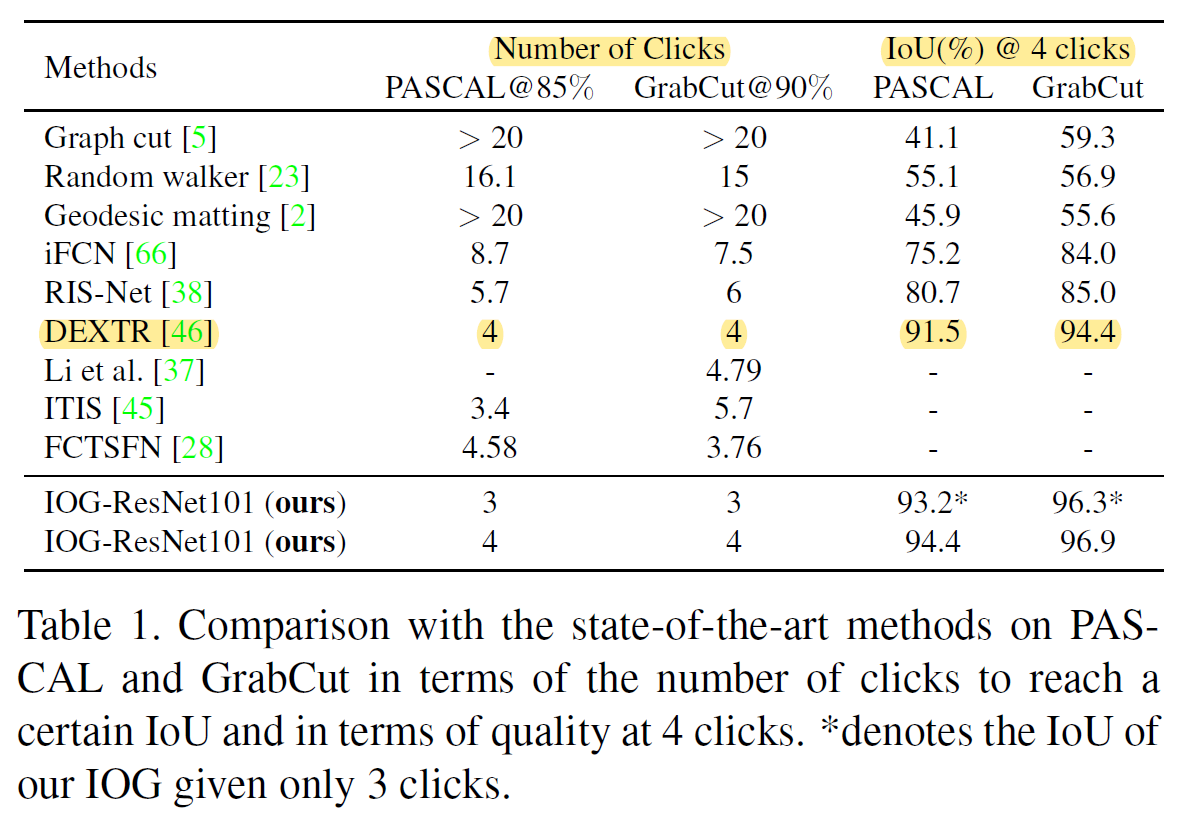
\includegraphics[width=\linewidth]{figures/chap31_comparison.png}
	\caption{Comparison with state-of-the-art methods.}
	\label{fig:ch3:sec1:comparison}
\end{figure}
